%This image depicts a structural mechanics diagram with three bars connected at a central node B, supported at points A, C, and D. A red force vector F is applied at node B. Dashed lines indicate the deformed configuration of the structure, with B' representing the displaced position of node B. The diagram also includes labels for axial stiffness (EA) and displacement components (uB, vB).
\documentclass[tikz,border=5pt]{standalone}
\usepackage{pgfplots}
\pgfplotsset{/pgf/number format/use comma,compat=1.16}
\usepackage[T1]{fontenc}
\usepackage[utf8]{inputenc}
\usepackage{stanli} % TikZ Library for Structural Analysis by Jurgen Hackl
\usetikzlibrary{calc,intersections,patterns}

\begin{document}
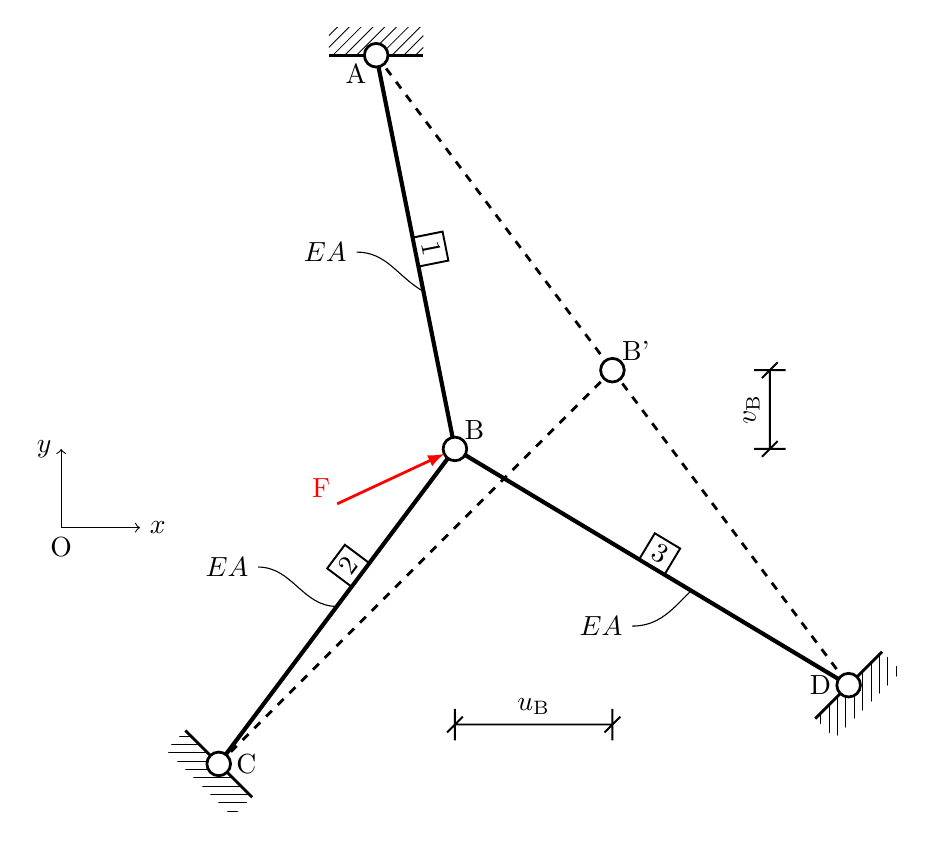
\begin{tikzpicture}[scale=1]
%\draw [help lines] (0,0) grid [step=1] (8,9); %useful for construction
% origin of the coordinates system
%coordinate system origin O
\draw (-2,3) node[below] {O};
%coordinates system
\draw[<->] (-1,3) node[right] {$x$}-|(-2,4) node[left]{$y$};
%point
\point{A}{2}{9};
\point{B}{3}{4};
\point{B'}{5}{5};
\point{C}{0}{0};
\point{D}{8}{1};
%beams
%left bar 1
\beam{2}{A}{B}[0][0];
%bottom left bar 2
\beam{2}{B}{C}[0][0];
%bottom right fixed support
\beam{2}{B}{D}[0][0];
%dashed line node B'
\beam{3}{A}{B'};
%bottom left bar 2
\beam{3}{B'}{C};
%bottom right fixed support
\beam{3}{B'}{D};
%left bar 1
\notation{4}{A}{B}[1];
%bottom left bar 2
\notation{4}{C}{B}[2][0.6];
%dashed line deformed structure
\notation{4}{D}{B}[3];
%supports
\support{3}{A}[180];
\support{3}{C}[-45];
\support{3}{D}[45];
%hinges
\hinge{1}{A}
\hinge{1}{B}
\hinge{1}{C}
\hinge{1}{D}
\hinge{1}{B'}
%load force
%red force vector F
\begin{scope}[color=red]
\load{1}{B}[205][1.5];
%red force vector F
\notation{1}{1.3,3.5}{F}[centered];
\end{scope}
%displacements
%horizontal displacement uB
\dimensioning{1}{B}{B'}{0.5}[$u_\mathrm{B}$];
%vertical displacement vB
\dimensioning{2}{B}{B'}{7}[$v_\mathrm{B}$];
%labels
\notation{1}{A}{A}[below left];
%central node B
\notation{1}{B}{B}[above right];
%dashed line deformed structure
\notation{1}{B'}{B'}[above right];
%bottom left fixed support
\notation{1}{C}{C}[right=1mm];
%bottom right fixed support
\notation{1}{D}{D}[left=1mm];
%bottom left fixed support
\draw (0.5,2.5) node[left]{$EA$} to [out=0,in=180] (1.5,2);
%left EA label
\draw (1.75,6.5) node[left]{$EA$} to [out=0,in=150] (2.6,6);
%bottom right EA label
\draw (5.25,1.75) node[left]{$EA$} to [out=0,in=225] (6,2.2);
% To-paths are really useful for drawing curved lines. The above
% to path is equal to:
%
% \draw[-latex,thick] (3.2,0.5) node[right]{$\mathsf{S_{1,2}}$}
%      ..controls +(180:.2cm) and +(up:0.25cm) .. (3,0);
% Internally the to path is translated to a similar bezier curve,
% but the to path syntax hides the complexity from the user.
\end{tikzpicture}
\end{document}